\section{Booster Return, Control and Actuation}
\label{sec:return}

The return controller commands the separated booster from separation to
touchdown through the phases of Section~\ref{sec:vehicle}: boostback
burn, return coast, entry burn, aerodynamic descent and landing burn
(\texttt{recovery.py}). Control is recomputed on a fixed
guidance period of $0.2\,\mathrm{s}$; throttle changes run through
$1\,\mathrm{s}$ smooth ramps, and the burn timing of the nominal run
appears in Figure~\ref{fig:thrust-profile}. Boostback and entry burns
run the three-engine set $(0,1,5)$; the landing burn runs the single
center engine. The legs deploy at landing ignition. The
controller feeds back the truth state and commands ideal attitude
moments --- class A project assumptions --- so the navigation solution is
deliberately not in the loop yet.

\begin{figure}[htbp]
\centering
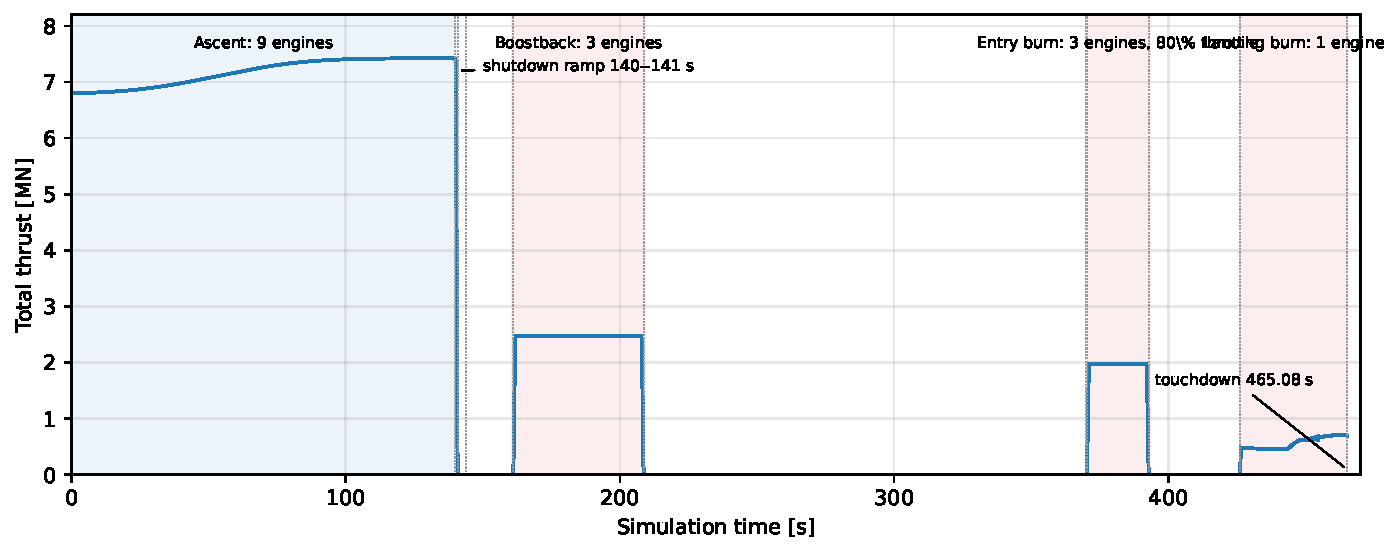
\includegraphics[width=\linewidth]{images/thrust_profile.pdf}
\caption{Total thrust of the nominal full-mission run (seed 1). The
booster burns are command-planned: boostback on three engines at full
throttle, the entry burn on three engines at $80\,\%$ throttle, and the
landing burn on the single center engine. Touchdown at
$t = 465.08\,\mathrm{s}$.}
\label{fig:thrust-profile}
\end{figure}

\subsection{Boostback: prediction and steering}

Boostback steering inverts a predicted landing miss. A reduced-order
ballistic predictor propagates the booster state forward in
$0.5\,\mathrm{s}$ steps with central gravity and rotating-frame
accelerations (Section~\ref{sec:environment}), the declared
\texttt{booster\_return} axial and crossflow coefficients
(Section~\ref{sec:aero}), and a prospective three-engine entry burn at the
declared altitude and throttle; the resulting predicted impact miss is
refreshed every second. During coast and the burn, the commanded
acceleration is
%
\begin{equation}
\label{eq:boostback-law}
\mathbf{a}_{\mathrm{cmd}} = -\,\frac{\hat{\mathbf{m}}}{8\,t_f}
\;+\; 0.8\,\hat{\mathbf{u}},
\end{equation}
%
where $\hat{\mathbf{m}}$ is the predicted miss vector, $t_f$ the ballistic
flight time and $\hat{\mathbf{u}}$ the local vertical. The burn stops on
the first satisfied condition: the predicted miss norm falls below
$500\,\mathrm{m}$ (the "predicted ballistic miss tolerance"), or the
burn duration leaves its $10$--$60\,\mathrm{s}$ planning window, or its
budget cap is reached. In the nominal run the boostback ends at
$208.81\,\mathrm{s}$ on the planning cap.

\subsection{Entry burn and aerodynamic descent}

Entry ignition requires the descending-through-$45\,\mathrm{km}$
condition plus the restart guards (budget, attitude, propulsion). During
the burn the commanded acceleration is a $30\,\mathrm{m/s^2}$ retrograde
bias plus lateral correction,
$\mathbf{a}_{\mathrm{cmd}} = 30\,\hat{\mathbf{u}} +
(\mathbf{v}_{d,h} - \mathbf{v}_h)/8 - \mathbf{a}_{\mathrm{aero}}$, toward
the desired horizontal velocity
$\mathbf{v}_{d,h} = -\mathbf{e}_h/(t_f + 25\,\mathrm{s})$ that nulls the
target error over the remaining flight. The burn ends when the speed
reaches $500\,\mathrm{m/s}$ or its budget cap fires. Through the
aerodynamic descent the vehicle holds a retrograde attitude above
$8\,\mathrm{km}$ and transitions to vertical attitude below, with the
grid fins available for residual moment demand.

\subsection{Landing burn and touchdown}

Landing ignition is predictive: a reduced-order stopping simulation
propagates the booster in $0.1\,\mathrm{s}$ steps with the landing
aerodynamic model, tilted thrust scaled by the ignition factor $1.05$,
and the current throttle amplitude; when the simulated stop leaves the
vehicle no more than the declared $1.5\,\mathrm{km}$ clearance allowance
above the ground, the burn ignites (nominal: $426.16\,\mathrm{s}$). The
guidance law is a second-order polynomial descent to the target with
terminal vertical velocity $v_{t} = -0.5\,\mathrm{m/s}$:
%
\begin{equation}
\label{eq:landing-law}
\mathbf{a}_{\mathrm{cmd}} = \frac{6\,(\mathbf{r}_{\mathrm{goal}} -
\mathbf{r})}{t_{go}^2} - \frac{4\,\mathbf{v}}{t_{go}}
- \frac{2\,v_t}{t_{go}}\,\hat{\mathbf{u}}
- \mathbf{g} - \mathbf{a}_{\mathrm{aero}},
\end{equation}
%
with $t_{go}$ from the current altitude and sink rate. The lateral
component of Equation~\eqref{eq:landing-law} is clamped by the
$20^{\circ}$ tilt limit, which tapers to a $4^{\circ}$ terminal attitude
below the $20\,\mathrm{m}$ hold height. Touchdown is the ground contact
of the lowest leg tip --- four assumed tips, $1\,\mathrm{m}$ below the
base at a $3.5\,\mathrm{m}$ radius --- and the run loop resolves the
contact instant by bisection; the acceptance criteria of
Table~\ref{tab:landing-limits} are evaluated at that instant. The
command path from guidance through actuation to the applied forces and
moments is completed by the actuator layer.

\begin{table}[htbp]
\centering
\begin{tabular}{lrr}
\toprule
Landing acceptance metric & Limit & Result (nominal run) \\
\midrule
Vertical speed & $\le 2\,\mathrm{m/s}$ & $0.497\,\mathrm{m/s}$ \\
Horizontal speed & $\le 1\,\mathrm{m/s}$ & $0.902\,\mathrm{m/s}$ \\
Target error & $\le 10\,\mathrm{m}$ & $3.306\,\mathrm{m}$ \\
Tilt & $\le 5^{\circ}$ & $0.535^{\circ}$ \\
Angular rate & $\le 1\,^{\circ}/\mathrm{s}$ & $0.013\,^{\circ}/\mathrm{s}$ \\
\bottomrule
\end{tabular}
\caption{Provisional project acceptance limits for a near-stationary
upright contact (class A; not Falcon~9 certified limits) and the nominal
run's contact metrics at $465.083\,\mathrm{s}$.}
\label{tab:landing-limits}
\end{table}

\subsection{Force and moment allocation}

Each commanded acceleration is converted to a bounded force allocation:
a numerical solver chooses the nose direction within the active tilt
envelope, the engine count and the throttle such that the resultant of
engine thrust (vacuum thrust minus exit-area ambient pressure at the
engine station) and the modelled aerodynamic reaction matches the
requested force; the corresponding ideal attitude moment drives the
vehicle toward that nose direction, with the moment authority capped at
$2\,\mathrm{MN\,m}$ during burns and $200\,\mathrm{kN\,m}$ in coast. Grid
fins carry residual moment demand beyond the virtual-vector authority,
mainly roll. Control gains: attitude $k_p = 1.0$,
$k_d = 2.0$; landing lateral $k_p = 0.0576$, $k_d = 0.48$; landing
attitude $k_p = 1.5$, $k_d = 6.0$.

% +++++ PENDING SUBSECTION (see ../docs/flags.md FL-2): Actuator layer.
% To be written LAST, against the final Actuators.py implementation:
% command path from the recovery/attitude laws through actuator dynamics
% to TVC gimbal (5 deg limit) and grid-fin rate/travel (+/-20 deg)
% forces and moments, ramp/rate limits, and its tests. Ground every
% statement in the implemented code; scope to what exists; then re-run
% the test suites, re-generate the nominal run and update
% Figure~\ref{fig:thrust-profile} if behavior changed.
